\subsubsection{Referencespænding}
Der skal ved offset- og komparatorblokken forsynes med en konstant spænding, da spændingen skal anvendes som sammenligningsgrundlag ift. andre signaler. Denne spænding kaldes en referencespænding. Referencespændingen består af en spændingsforsyning, en modstand og en spændingsreference diode. Der anvendes en referencediode af typen LM385, som både findes som $1.2$V og $2.5$V. Et eksempel på en opsætning af en spændingsreference kan ses på figur \figref{fig:Spaendingsreference}.

\begin{figure}[H]
	\centering
	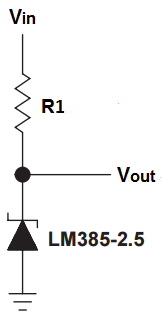
\includegraphics[scale=1.0]{figures/cProblemloesning/ReferenceEksempel}
	\caption{Figuren illustrerer et eksempel på opsætning af et kredsløb for en spændingsreference med LM$385$. Figuren er en revideret udgave fra kilden. \cite{Instruments2005}}
	\label{fig:Spaendingsreference}
\end{figure}

For at udregne værdien af modstanden i kredsløbet, anvendes følgende generelle formel:
\begin{equation}
R=\dfrac{V_{forsyning}-V_{Reference}}{I_{Z(min)}}
\end{equation}
Hvor V_{forsyning} er forsyningsspændingen som sendes ind i kredsløbet, V_{Reference} er den referencespænding der skal sendes ud af systemet og I_{Z(min)} er den strøm, systemet minimalt forbruger.

\textbf{Test af referencespænding}


 